\section{Organización del modelo de información}

    El modelado de la estructura de la información del \paear utiliza la notación de los diagramas de clases de UML. En él se plasman las estructuras de información y las relaciones entre ellas.

    En un diagrama de clases se modelan las estructuras o \cdtRef{gls:entidad}{entidades del negocio} como rectángulos con dos compartimentos: En el primero se coloca su nombre y en el segundo se listan sus atributos. Por otro lado las relaciones que se representan son de dos tipos:	

    \begin{Citemize}
	\item Asociación, representada mediante una linea continua. Esta se utiliza para indicar que la información de un extremo de la línea está ``asociada'' con la del otro. Dicha asociación puede señalar que una entidad ``compone'' a la otra o que se le ``agrega''.
	
	Por ejemplo, una entidad de dominio público es ``persona'' la cual se ``compone'' de otra entidad llamada ``ojos'', sin embargo, la misma entidad ``persona'' puede tener un ``auto''. Esta última relación sería una asociación de ``agregación'' dado que el quitarle o cambiarle el ``auto'' a la ``persona'' no la mutila ni deja de ser una ``persona'', a diferencia de lo que pasa con los ``ojos''.
	
	Además, las relaciones de ``asociación'' suelen especificar una ``cardinalidad''. La cardinalidad indica las cantidades que rigen dicha relación. La cardinalidad se indica como: de uno a muchos, de uno a uno, de muchos a uno o de muchos a muchos. Por ejemplo, una ``persona'' tiene dos ``ojos'', pero cada ojo pertenece sólo a una ``persona''. Esta asociación tiene una cardinalidad de ``uno a muchos'' (que significa que una persona puede tener muchos ojos y un ojo pertenece sólo a una persona) o de ``uno a dos'' (Mas específicamente que una persona tiene dos ojos). 
	
	\item Herencia, representada mediante una línea terminada en una punta triangular. En este caso la relación indica una especialización entre las entidades, es decir que la  entidad del lado contrario al de la flecha es una ``especialización'' de la entidad del otro extremo.
    \end{Citemize}

    La especificación del modelo de información incluye:
    \begin{Citemize}
	\item Una descripción de cada una de las entidades.
	\item Una descripción de los atributos que conforman las clases.
	\item Una descripción de la relación entre las clases.
    \end{Citemize}

%    Dada la cantidad de conceptos en esta especificación, se ha organizado en secciones por campo de conocimiento como lo muestra la figura~\ref{fig:modeloInformacionGeneral}:\\
	
    % \begin{figure}[htbp!]
    % 	\begin{center}
    % 		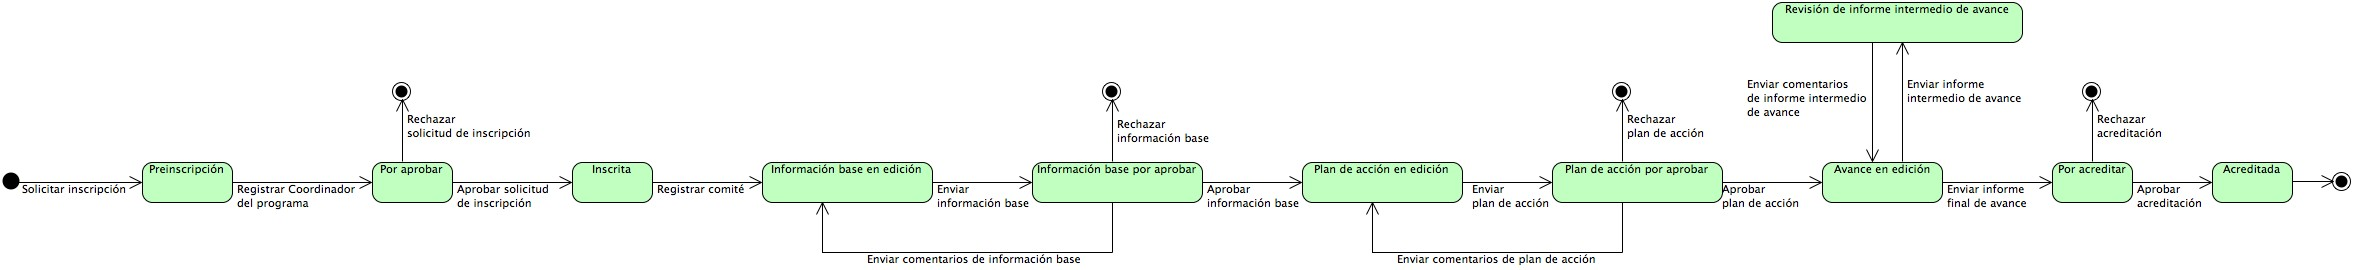
\includegraphics[width=0.9\textwidth]{images/clases/general}
    % 		\caption{Estructura del modelo de infomación.}
    % 		\label{fig:modeloInformacionGeneral}
    % 	\end{center}
    % \end{figure}

%    Las entidades se encuentran coloreadas principalmente con el tono del paquete al que pertenecen, y los atributos de términos propios del negocio se modelan mediante entidades de color gris. La definición de estas se encuentra en el glosario de términos (sección~\ref{sec:glosario} pág.~\pageref{sec:glosario}).
